\documentclass[12pt]{article}
% This first part of the file is called the PREAMBLE. It includes
% customizations and command definitions. The preamble is everything
% between \documentclass and \begin{document}.

\usepackage[margin=1in]{geometry}  % set the margins to 1in on all sides
\usepackage{graphicx}              % to include figures
\usepackage{amsmath}               % great math stuff
\usepackage{amsfonts}              % for blackboard bold, etc
\usepackage{amsthm}                % better theorem environments

\usepackage{rotating} % for sideway table
\usepackage{xcolor}
\usepackage{hyperref}
\hypersetup{
    colorlinks,
    linkcolor={red!50!black},
    citecolor={blue!50!black},
    urlcolor={blue!80!black}
}
\usepackage{cleveref} % Reference
\usepackage{enumitem} % nosep

\usepackage{array,tabularx}

\newenvironment{conditions*}
  {\par\vspace{\abovedisplayskip}\noindent
   \tabularx{\columnwidth}{>{$}l<{$} @{${}={}$} >{\raggedright\arraybackslash}X}}
  {\endtabularx\par\vspace{\belowdisplayskip}}
  
\usepackage{float}
\restylefloat{table}

% various theorems, numbered by section

\newtheorem{thm}{Theorem}[section]
\newtheorem{lem}[thm]{Lemma}
\newtheorem{prop}[thm]{Proposition}
\newtheorem{cor}[thm]{Corollary}
\newtheorem{conj}[thm]{Conjecture}
\newtheorem{hyp}{Hypothesis}

\DeclareMathOperator{\id}{id}

\newcommand{\bd}[1]{\mathbf{#1}}  % for bolding symbols
\newcommand{\RR}{\mathbb{R}}      % for Real numbers
\newcommand{\ZZ}{\mathbb{Z}}      % for Integers
\newcommand{\col}[1]{\left[\begin{matrix} #1 \end{matrix} \right]}
\newcommand{\comb}[2]{\binom{#1^2 + #2^2}{#1+#2}}

% bibliography
\usepackage{natbib}
\bibpunct{(}{)}{;}{a}{}{,} % no comma between author and year

\title{Prospectus: The political determinants of FDI technological spillover and corruption}
\author{Anh Le}


\begin{document}
\maketitle

\section{Empirical Puzzle}
In recent decades, foreign direct investment (FDI) global flow has steadily increased, rising to over \$1.5 trillion dollars in 2014. For developing countries, FDI flow is also remarkably robust to global downturn, leading to enthusiastic endorsement by major international organizations as a key factor to economic development (\Cref{fig:globalfdi}).\footnote{http://www.imf.org/external/pubs/ft/fandd/1999/03/mallampa.htm, http://www.weforum.org/reports/foreign-direct-investment-key-driver-trade-growth-and-prosperity-case-multilateral-agreement} This assumption is also shared widely within political science, where much of the literature starts with the assumption that countries want to seek FDI for its many benefits. The question that these works focus on is \textit{how} countries can attract FDI, not \textit{whether} they want to do so \citep{Jensen2003, Li2003, Li2006, Ahlquist2006}.\footnote{Two recent exceptions are \citet{Pinto2013, Pandya2013}, which are the first to investigate the demand for FDI.} 

\begin{figure}[!ht]
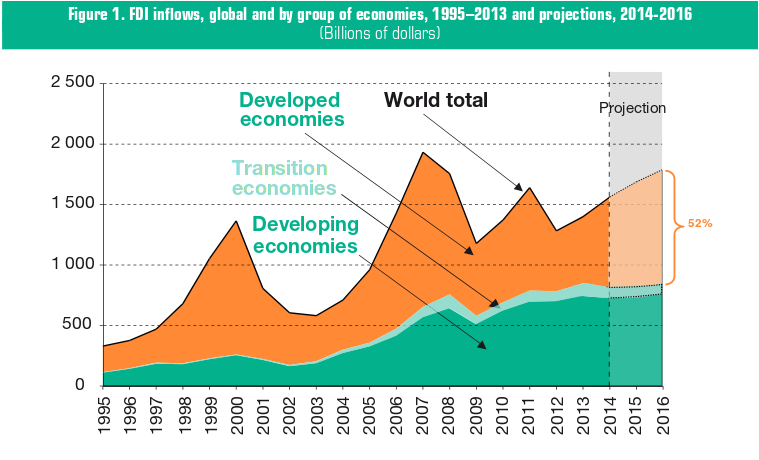
\includegraphics[width=\textwidth, height=\textheight,keepaspectratio]{../figure/global_fdi}
\caption{Source: World Investment Report, 2014}
\label{fig:globalfdi}
\end{figure}

Underlying this mode of thinking is the assumption that FDI brings various benefits to developing countries, including capital and employment. However, the most important promise that FDI holds to growth is the spillover of productivity between foreign firms and domestic firms. This can happen if local firms hire workers that were trained in a foreign firms, improve productivity through backward and forward linkages, or imitate foreign technology. According to growth theory, it is FDI's spillover, not capital or employment, that brings the technological innovation that is requisite for economic growth \citep{Findlay1978}. In this view, FDI is also a public good, providing spillover benefits to the local firms in ways that foreign firms do not take into account in their private calculations. This provides the justification for countries' using investment incentives to rectify the undersupply of FDI, closing the gap between private and social returns. 

Despite this prevailing view, there is little conclusive evidence of FDI having a positive effect on growth \citep{Nair-Reichert2001, Carkovic2002} or poverty reduction \citep{Guerra2009} (\Cref{fig:fdipoverty}). A substantial literature has developed to explain this puzzle, concluding that the growth-enhancing and spillover effect of FDI is conditional on the absorptive capacity of local firms. Cross-nationally, scholars find that FDI is more likely to have a positive growth effect when the technological gap between the local and foreign firms are small \citep{Nunnenkamp2004} and when host countries have strong financial and institutional development \citep{ Durham2004}. Similarly, absorptive capacity, measured by the level of schooling in host economy, conditions the transfer of technology between foreign and local firms across regions in China \citep{Fu2008} and countries in Latin America \citep{Willem2004}.

\begin{figure}[!ht]
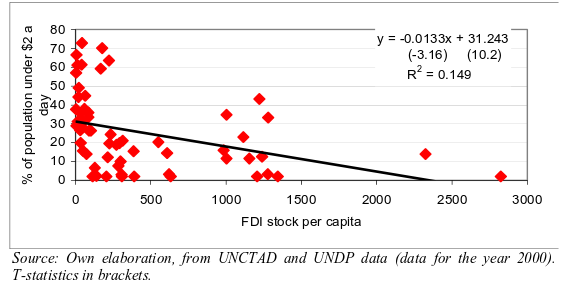
\includegraphics[width=\textwidth, height=\textheight,keepaspectratio]{../figure/fdi_poverty}
\caption{Relationship between FDI and poverty}
\label{fig:fdipoverty}
\end{figure}

Despite the resounding conclusion that the effect of FDI is highly conditional and that investment incentives do not work, why do countries still fixate so much on bringing in FDI instead of developing local absorptive capacity \citep{Blomstrom2002}? For example, Ireland provided foreign investors with lower tax rate, lower land price, and cash grants for R\&D that do not need to be repaid. China also used a tax holiday (two years of no tax and three year of half the normal tax rate) in special economic zones to attract more foreign firms \citep{Telford2001}. We see the same widespread use of investment incentives in Southeast Asia \citep{Fletcher2002}. In Vietnam, the race to offer incentives to foreign firms rages on even among sub-national units, as provincial governments defied the central government's directive and offered extra-legal incentives to FDI firms \citep{Vu2007}. Not only do these measures not work in attracting more FDI, they also deprive countries of revenues that could be spent on improving the local labor quality and investment climate, which are much more conducive to spillover effect and growth.

Thus, my dissertation project focuses on this empirical puzzle: if the positive effect of FDI is uncertain, why is there so much focus on attracting it? If developing absorptive capacity is so crucial to making FDI growth-enhancing, why is it often neglected? To understand this puzzle, I propose that we need to take into account the calculus of the individual bureaucrats and government officials, who may be more interested in the potential rents from foreign firms than the spillover and growth-enhancing effect of FDI. This is a potential reason why we often see countries (i.e. government officials) being so enthusiastic about attracting FDI, yet not so passionate about developing the local capacity that enables FDI to actually have a positive effect on growth.

\begin{figure}[!ht]
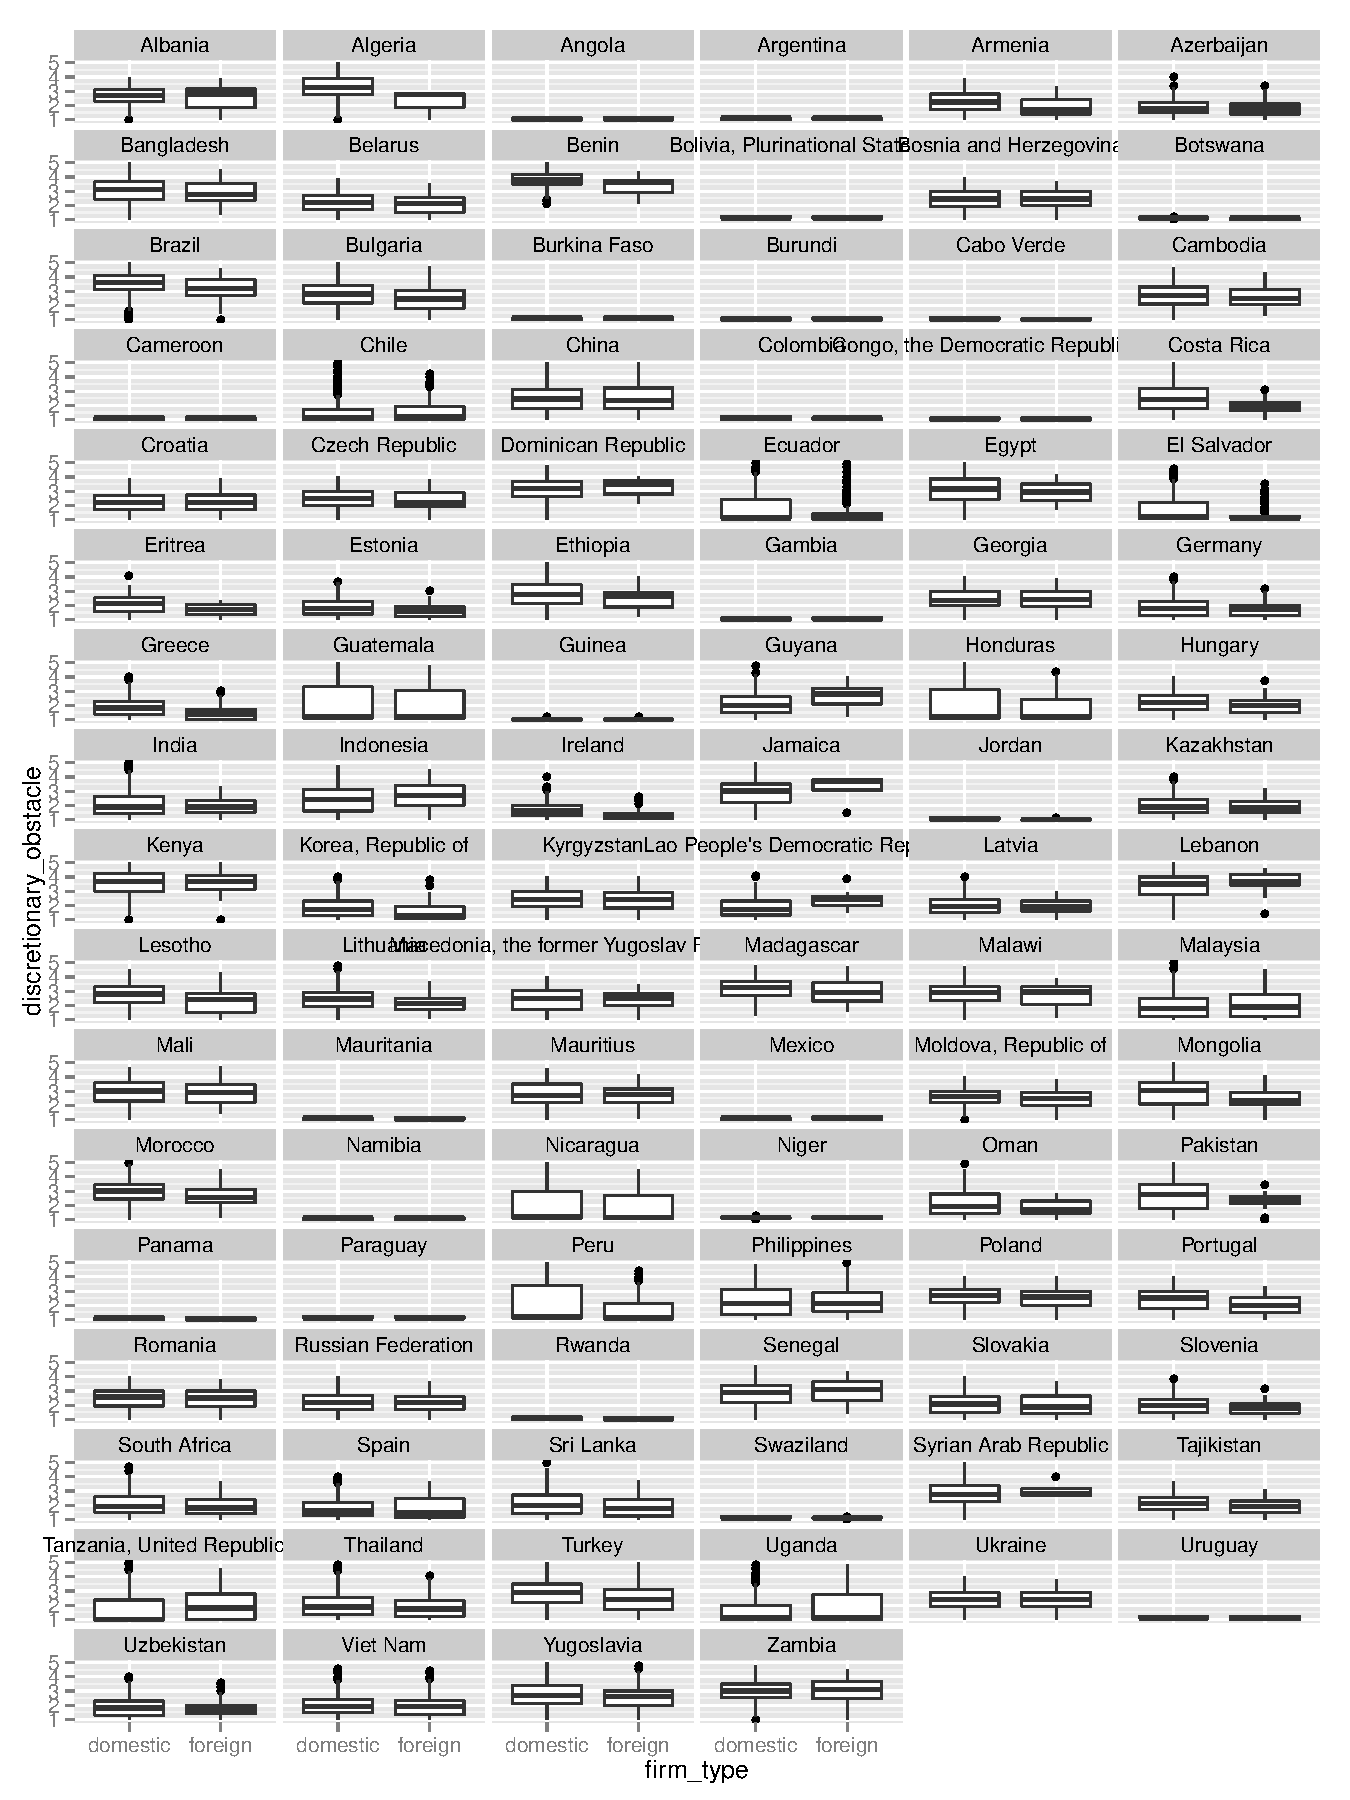
\includegraphics[width=\textwidth, height=\textheight,keepaspectratio]{../figure/fdi_domestic_treatment}
\caption{The treatment of FDI and domestic firms across countries}
\label{fig:fdi_domestic_treatment}
\end{figure}

Starting with this empirical puzzle, my project also sheds light on various related issues. First, it investigates the collusion of FDI firms and host countries' officials, a understudied phenomenon as the existing literature often assumes a foreign firm trying to fend off extortion and harassment from host countries. Second, it examines the political drivers behind private sector development, an issue whose welfare impact is well-known yet whose political determinants are ill-understood. Third, my project looks at the treatment of foreign firms versus domestic firms from a fresh angle. The majority of political science literature has considered FDI the underdog, unfamiliar with the location, susceptible to expropriation, and threatened by the lobbying effort of domestic firms. However, when FDI firms are big and resourceful, they can be an equal partner in the collusive relationship with corrupt officials to the detriment of the domestic sector.


\section{Stylized Facts}
In this section, I present some evidences that motivate the puzzle.

\begin{itemize}
	\item The spillover effect of FDI on growth is highly variable. For example, FDI is found to be growth-enhancing in East Asia, but not in Latin America \citep{Zhang2001}. Similarly, the effect of FDI on domestic investment also varies across countries and regions. FDI is found to crowd in investment in some countries (e.g. Ghana, Senegal, South Korea, Pakistan, Thailand, etc.) but crowd out in others \citep{Agosin2005}.
	
	\item Despite the prevalent concern with discrimination against foreign firms, the Wold Bank Enterprise Survey finds that foreign firms actually face fewer obstacles while doing business \citep{Batra2003}. The gap in the treatment of foreign and domestic firms also varies across countries (\Cref{fig:fdi_domestic_treatment}).
	
	\item The correlation between corruption and FDI is negative. However, there is a lot of unexplained variance at the high end of FDI. Countries with low level of FDI are always very corrupt, but countries with high level of FDI can be as well (\Cref{fig:fdi_corruption}).
	
	\begin{figure}[!ht]
	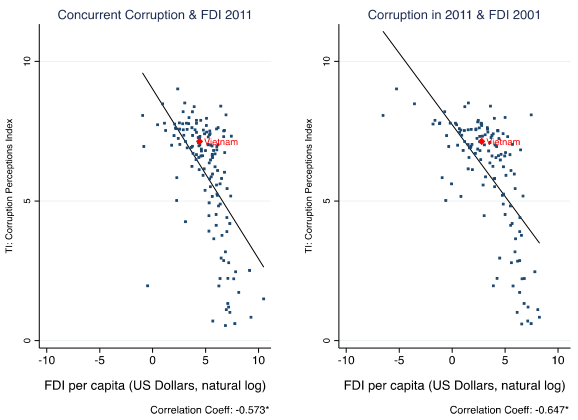
\includegraphics[width=\textwidth, height=\textheight,keepaspectratio]{../figure/fdi_corruption}
	\caption{Source: \citep{Malesky2015}}
	\label{fig:fdi_corruption}
	\end{figure}
\end{itemize}

A closer look into the level of corruption across industries also suggests a negative relationship between spillover and bribe. According to the \citet{TransparencyInternational2011}'s Bribe Payer Index, which measures the propensity of firms from industrialized countries bribing abroad, the most corrupt sectors are public works contracts, utilities, real estate, oil and gas, and mining. These sectors are most vulnerable to corruption due to a lack of competition and a high level of government involvement. They also tend to be less conducive to spillover due to the winner-take-all structure of the industry \citep[138]{UNCTAD2001}. For example, in real estate, utilities, or mining, if scarce resources and contracts can only be won by large foreign firms, then these firms will capture the rent and perpetuate their market power while relegating local contractors to low-value added tasks.

In contrast, the least corrupt sectors are agriculture, light manufacturing, civilian aerospace, IT, and banking and finance. Among these, some are high tech industries (e.g. aerospace, IT) that governments may prioritize to facilitate spillover. Others have low barriers to entry and a divisible production process, both of which are conducive to domestic sourcing (e.g. agriculture, light manufacturing) \citep{TransparencyInternational2011}.

Beyond these broad strokes, the relationship between spillover and corruption emerges in more granularity within the same sector and across countries. For example, despite the stereotype as a high corruption, low spillover sector, the mining industries in Chile, Ghana, and Mozambique have substantial variation of spillover according to the host country's level of corruption. According to the \citet{TransparencyInternational2014}'s Corruption Perception Index, Chile, Ghana, and Mozambique rank 21, 61, and 119 out of 175 countries on control of corruption. Correspondingly, according to surveys of mining firms, Chilean foreign mines ``have the greatest proportion of domestic suppliers and carry out more valued-added activities in-country than [foreign mines] in Ghana and particularly more than in Mozambique'' \citep[127]{Farole2014}. The high level of FDI spillover in Chilean mining may be due to its developed economy and competent base of local suppliers. However, this does not explain the difference between Mozambique and Ghana, two countries with a similar level of GDP per capita.

Importantly, Ghana and Mozambique differ not only in the level of spillover, which can be influenced by economic forces outside the government's strategic decision. In addition, the two governments also diverge in their policies to promote supply chain linkages between foreign and domestic firms. In Ghana, the government worked with the private sector to develop regulations that put real teeth into the local content requirements in the Ghana Minerals and Mining Act (2006). According to these regulations, foreign mining firms are required to develop a five-year local procurement plan, including targets and strategies to develop domestic supplier capacity. These is also clear evidence that the government enforces these rules by striking at the profitability of the firms: when bids are within two percent of prices, the bid with the highest local content shall be selected. In stark contrast, Mozambique shows no commitment to local supplier development either in its Mining Law (2002) or Mining Regulations (Decree no.62/2006) \citep[137]{Farole2014}.

This example shows that if a government wants to induce spillover from foreign firms, it can. Even though policies that affect the profitability of the foreign firms, such as local content requirement, are technically not allowed under the national treatment principle of the WTO, there are many loopholes and little enforcement \citep{Hufbauer2013}. Indeed, Ghana itself has been a WTO member since 1995 and a GATT member since 1962. Therefore, the interesting question is not whether the government can extract spillover from FDI, but under what conditions would it want to do so.


\section{Roadmap}
In the next sections

\section{Theory}
\subsection{``Price of spillover'' sectoral variation}

As implied in the theory section, when the ``price'' of spillover is high (i.e. it is difficult to obtain spillover given the country's absorptive capacity or sector-specific characteristics), the government official would choose a bundle that has more private benefit than spillover. 

PICTURE

Here I focus on industry-specific characteristics that either facilitate or hinder spillover. Due to its divisible process, manufacturing firms tend to engage more local suppliers and generate more spillover effect than primary and tertiary sectors. In addition, there is a wide variation across industries within a sector to be exploited as well. For example, in manufacturing, food processing can have a high amount of spillover due the sourcing of raw materials and packaging, whereas in textile and automotive industries (which require high level of technological sophistication), it is harder for foreign firms to work with local suppliers. Similarly, in tertiary sectors, finance, trading, tourisms and utilities are is generally not divisible into discrete stages to subcontract. Yet service industries such as retailing and construction have more opportunities for input suppliers (cite).

This leads us to the following hypothesis:

\begin{quote}
Hypothesis: Government official will pursue less private benefits from firms in industries where it is easier to generate spillover
\end{quote}

While such variation across industry is clear conceptually, measurement is thorny given the many factors that can affect the potential for spillover. In addition, there is an endogeneity problem as the potential for spillover may itself be affected by the level of rent-seeking of that industry. For example, an industry plagued by collusive relationship between the official and the foreign firms does not offer an enabling environment that allows private firms to develop their absorptive capacity. The endogeneity problem is compounded if the official strategically invests to improve absorptive capacity, in which case it is not even clear which direction is our estimate biased.

To address both of these measurement and endogeneity issues, I will use the variation in technological spillover across industries in the United States as the instrumental variable.\footnote{The United States is considered due to its high quality economic data. Alternatively, for each country, I can use a comparable country in the same region or the same developmental stage to formulate the instrument} The assumption is that the level of technological spillover in a US industry only correlates with the level of bribe in another country's industry through the latent factor that is the industry-specific potential for spillover.

\subsection{``Price of private benefit'' firms ability to bribe}

As implied from the theory, when the ``price'' of private benefit is high (i.e. it is costly for the firm to offer the official private benefit), the official would choose a bundle that has less private benefit.

This theoretical claim generates many substantive predictions that we can test, each involving a factor that affect the cost of bribing for firms. For example, foreign firms that come from a corrupt home countries may have more experience with bribing and thus would incur less information cost if they bribe.

Here I focus on the Phase 3 (Enforcement) of the OECD Anti-Bribery Convention (ABC) as an exogenous increase in the cost of bribing for foreign firms in Vietnam. In December 1997, all members of OECD and an additional five non-members, accounting for nearly 61\% of world trade, signed the ABC. The ABC criminalizes the bribery of foreign public officials and upholds its principles with a peer-monitoring system, in which member countries visit and review one another's legislation and implementation. According to legal experts, these reports are often quite harsh and effective in shaming countries into improving their practices \citep{Tyler2011}.

Important for my research design, in December 2009 the OECD's Working Group on Bribery (WGB) annouced that following Phase 1 and 2 (Evaluation and Assessment) there would be a Phase 3 (Enforcement). The goal of Phase 3 is to continually monitor countries' anti-bribery practices and to exhort inactive enforcers. Noticeably, Phase 3 also removed a previous exception that allowed firms to make ``small facilitation payment'' \citep{Strauss2013}. Researchers have argued that following the announcement of Phase 3, member countries ramped up enforcement to avoid a negative review, and causing their firms to reduce bribery abroad \citep{Malesky2015b}. 

Given that FDI to Vietnam only accounts for a small fraction of OECD countries' total foreign investment, it is plausible that Vietnam is not a major factor driving the initiation of Phase 3. Therefore, the announcement of Phase 3 serves as an exogenous shock to the cost of bribery for firms from ABC member countries. With OECD firms being reluctant to offer bribes, we expect corrupt officials to become uninterested in OECD firms. Post 2009, OECD firms would be attractive only to non-corrupt officials for their developmental impact, and we should observe them having more spillover effect.\footnote{An alternative design looks at the difference between OECD and non-OECD firms that \textit{enter} Vietnam pre- and post-2009. This design will have fewer firms in the sample but could be more appropriate if we think that the spillover-bribe bundle is negotiated at the time firms enter Vietnam and is hard to change later, even with the ABC coming into effect. If so, the change in level of spillover and bribe is caused by the change in the official's selection of firms instead of the adjustment in behaviors of existing firms after 2009.}

With 2009 as an exogenous shock we have a difference-in-difference design. First, we estimate the difference in spillover between OECD and non-OECD firms, pre-2009. We then find the same difference in spillover post-2009. Subtracting these two differences, we can estimate the effect of corruption on the level of spillover.

I sum, I have the following hypothesis:

\begin{quote}
Hypothesis: The Phase 3 (Enforcement) of OECD's Anti-Bribery Convention causes firms from member countries to have more spillover and pay less bribe.
\end{quote}


\subsection{Time horizon of officials}

As implied by the theory above, an official with a longer time horizon would choose a bundle with more spillover, whereas an official with a short time horizon would choose a bundle with more private benefit.

To get a handle on the time horizon of the official, we need to know the options provided to the official within the country's political economic system. Such is a big and difficult question to study with a cross-national design due to an insurmountable degree of endogeneity stemming from unobservable and unmeasurable differences across political systems. Therefore, at this step, I focus on the case of Vietnam, whose sub-national variation in FDI flow and private sector development serve as an excellent testing ground. Again, here I focus on bribe and informal fees as the main form of private benefit for officials. Such constraint is not problematic for the case of Vietnam, where the authoritarian system means that officials are not offered campaign contribution and where revolving door jobs are non-existent.

\subsubsection{The effect of time horizon on the choice of Vietnamese provincial officials} 

The relative weight assigned to spillover versus bribe by the Vietnamese provincial officials is determined by the principal-agent relationship between Vietnam's central and the provincial governments. On the one hand, the central government (i.e. the principal) cares more about the spillover effect of FDI and uses promotion to reward local officials that attract high-spillover FDI. On the other hand, local officials (i.e. the agent) have more opportunities to engage in corruption with foreign firms, and should they decide that the private benefit of corruption is greater than that of promotion, they will prioritize foreign firms that bring bribes over those that have high spillover effects.

The reason behind such difference in the preference of central and local governments is the fact that FDI projects are approved and managed at the provincial level. While the central law may be uniform in the book, its implementation varies widely across sub-national units in Vietnam \citep{Meyer2005}.\footnote{Vietnam's sub-national variation in implementation generalizes well to other cases, such as China \citep{Thun2006}} Therefore, the provincial government holds valuable services for sale to foreign firms. In contrast, the central government is more removed from direct contact with FDI firms and thus less likely to benefit from corruption than provincial leaders. 

In addition, the central government is much more concerned with overall economic growth, which is central to the longevity of the regime \citep{Malesky2008}. It wants to attract high-spillover FDI and uses promotion to reward local officials that accomplish this goal. On the other hand, each provincial leader is incentivized to free-ride on the developmental effort of other provinces and of the central to keep the entire regime stable. Therefore, local officials value the spillover effect of FDI only insofar as the opportunities for promotion that it brings.

Fortunately for the central government, the principal-agent problem in this context is partially solved because monitoring is not too difficult. Indeed, the central government can observe the economic performance of the provinces and use personnel management to punish and reward provincial officials \citep{Sheng2007, Li2005}.\footnote{\citet{Shih2012} recently argue that economic performance does not matter to cadre promotion. However, they investigate all members of the Chinese Central Committee, including the central party apparatus, the army, and the central economic bureaucracy. These actors are not the important decision-makers in our theory.} Therefore, the principal-agent problem is only severe when provincial officials are not interested in further promotion to the central government, i.e. when the local official's time horizon is short. This suggests that there will be a variation in the level of FDI's spillover effect across provinces according to provincial officials' interest in promotion. In the research design, I use fuzzy regression discontinuity (RD) exploiting the mandated retirement age of Vietnamese officials, arguing that those that are in their last term have shorter time horizon and less interest in promotion. 

By looking at this variation in the career interest of provincial officials, my theory contributes a fresh angle to the current literature on the relationship between decentralization and corruption. So far, scholars have only postulated a one-way relationship: either decentralization increases bribery \citep{Fan2009} or reduces it \citep{Guerra2009}. In my model, how decentralization affects corruption is conditional on the local officials' interest in the promotions offered by the central as carrots.


Three key assumptions in the theory above deserve further examination:
\begin{enumerate}
\item Why wouldn't Vietnam's central government worry that a developed private sector may lead to social change that ultimately undermines its rule?

First, there is a large scholarship showing that authoritarian regimes are very adept at using institutions to manage regime outsiders in general and business in particular \citep{Gandhi2006, Gandhi2008, Wright2008, Le2015}. Second, if the legitimacy of the regime rests heavily on delivering economic growth, then the short-term risk of an economic downturn creating instability features much more prominently than the long-term concern with social changes. Third, it is possible to foster economic growth while restricting political freedom (e.g. Singapore). Indeed, growth can make a regime, both democratic and authoritarian, more stable, and creates room for political control \citep{Przeworski1997}.

\item Why don't provincial leaders seek rent from the domestic sector? 

First, Vietnam's private sector was very small when FDI was first allowed into Vietnam. The size and the profitability of the average domestic firm is still smaller than those of foreign firms today. Therefore, there are both fewer rents and more coordination problems if provincial officials want to seek rents from domestic firms. Second, ironically, if officials want to grow the private sector for future rent-seeking, they must promote an enabling business environment that are free from rent-seeking. In contrast, engaging in corruption with large and existing FDI firms is much more convenient. Essentially, corrupt provincial officials have shifted the cost of building a thriving domestic sectors to the home countries of FDI firms and now extract rents from the high productivity and high profitability of these firms. 
\end{enumerate}

In sum, I propose a hypothesis about variation across Vietnam's provinces:

\begin{quote}
Hypothesis: In provinces whose leaders are in their last term before the mandated retirement age, there are more spillover and less bribe from the foreign firms.
\end{quote}


\section{Research Design}
\subsection{Measuring the main dependent variable: spillover effect}
\label{sec:measure_spillover}

\subsubsection*{Measuring spillover indirectly}

Similar to how growth economists start endogenizing technological change, FDI researchers investigate how technology spillover from FDI may happen instead of assuming its inevitability \citep{Romer1994}. Several channels for spillovers have been proposed, some of which suggest an indirect measure of technology spillover.

These channels are:
\begin{itemize}
	\item imitation:  private firms may reverse engineer a production or management technique \citep{Wang1992}, which is facilitated by backward linkage between local and foreign firms \citep{Javorcik2004}. This motivates my first measure of spillover effect: \% of private firms that participate in contracts with foreign firms.
	\item competition: similar to the effect of competition from arm's length trade on productivity, the presence of foreign firms in the domestic market put pressure on local firms to reduce inefficiency \citep{Glass2002}.
	\item export demonstration: foreign firms are more knowledgeable about exporting, which involves high fixed cost to set up a distribution and transport infrastructure, or learning about foreign taste and regulatory environment. Domestic firms can learn this ``export know-how'' from foreign firms \citep{Aitken1997}. This motivates my third measure of spillover effect: \% of private firms that export.
	\item skills acquisition: workers trained in foreign firms bring along their human capital when they move to domestic firms \citep{Djankov2000}. This presumes a healthy domestic sector that can offer competitive wages to workers.
\end{itemize}

Among these channels, \textit{imitation} and \textit{export demonstration} forms the theoretical basis of my two proxy measurements of spillover:
\begin{enumerate}
\item frequent business contacts between foreign and domestic firms,
\item percentage of domestic firms engaging in export
\end{enumerate}

\subsubsection*{Measuring spillover directly}

As standard in the economic literature that studies whether there is a spillover effect for FDI, we can also measure spillover directly. This is done in two steps \citep{VanBeveren2012}.

\begin{itemize}
\item First, measure the level of technology or productivity of a firm.

Level of technology: R\&D spending

Level of productivity: Consider the familiar Cobb-Douglas production function:

\begin{align}
Y &= AL^{\alpha}K^{\beta}
\end{align}

where $Y$ is value added, $A$ is total-factor productivity (TFP), $L$ is labor, and $K$ is capital. $y$, $L$, and $K$ are observable, while $A$ is not. Log transform both sides of the equation, we attain a linear form:

\begin{align} \label{eq:cobb_douglas_linear}
y &= a + \alpha l + \beta k
\end{align}

where the lowercase variables are the log-form of the uppercase variables (e.g. $y = \log(Y)$ and so on). \autoref{eq:cobb_douglas_linear} can then be estimated with OLS:

\begin{align} \label{eq:cobb_douglas_OLS}
y_i = \beta_0 + \beta_1 l_i + \beta_2 k_i + \epsilon_i
\end{align} 

where $\beta_0$ is the average total-factor productivity of all firms and $\epsilon$ is the firm-specific deviation from that mean. From the estimated coefficients of \autoref{eq:cobb_douglas_OLS}, we can estimate firm-level TFP as follows:

\begin{align}
a_i &= \hat\beta_0 + \hat\epsilon_i \\
A &= \exp^{\hat\beta_0 + \hat\epsilon_i}
\end{align}

\item Having estimated firm-level TFP (or technology), we then regress TFP (or technology) on the presence of FDI in a country / sector. FDI presence can be measured as:
\begin{itemize}
\item amount of FDI or number of foreign firms in a country (sector). This measure focuses on the horizontal, or intra-sector, linkage of FDI
\item number of foreign firms that the domestic firms are in contact with. This measure focuses on the vertical, or inter-sector, linkage of FDI
\end{itemize}
\end{itemize}


\subsection{``Price'' of spillover: sectoral and industry variation in potential for spillover}

As implied in the theory section, when the ``price'' of spillover is high (i.e. it is difficult to obtain spillover due to the country's absorptive capacity or sector-specific characteristics), the government official would choose a bundle that has more private benefit than spillover (\Cref{fig:price_of_spillover}). 

\begin{figure}[!ht]
	\centering
    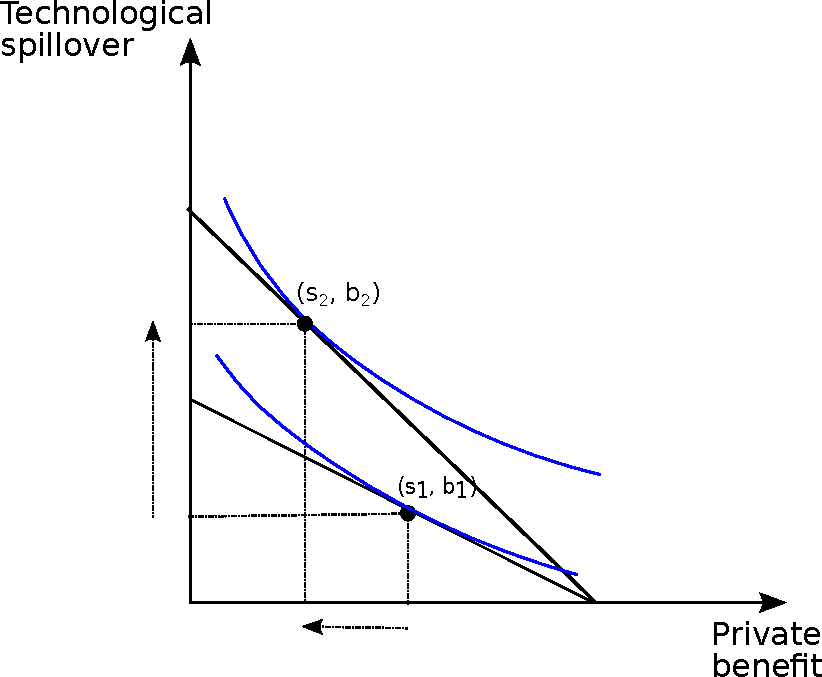
\includegraphics[width=0.75\textwidth, height=0.75\textheight,keepaspectratio]{../figure/price_of_spillover}
    \caption{As the ``price'' of spillover decreases, the official can get a larger amount of spillover given the same budget (i.e. the y-intercept of the budget constraint shifts up) Comparing the bundle $(s_1, b_1)$ and $(s_2, b_2)$, we see that the new bundle has more spillover and less bribe.}
    \label{fig:price_of_spillover}
\end{figure}

Here I focus on industry-specific characteristics that either facilitate or hinder spillover.\footnote{Absorptive capacity, or the ability of private firms to learn from their interaction with foreign firms, is also a very important factor in determining spillover. However, given the time-varying nature of absorptive capacity, not to mention the fact that official and firms can strategically invest to improve absorptive capacity, it is much harder to have a research design studying absorptive capacity that can claim exogeneity.} Due to the divisibility of its production process, manufacturing firms tend to engage more local suppliers and generate more spillover effect than primary and tertiary sectors. In addition, within each sector there is a wide variation across industries to be exploited as well. For example, in manufacturing, food processing can have a high amount of spillover due to the sourcing of raw materials and packaging, whereas in textile and automotive industries (which require high level of technological sophistication), it is harder for foreign firms to work with local suppliers. Similarly, in tertiary sectors, finance, trading, tourisms and utilities are is generally not divisible into discrete stages to subcontract. Yet service industries such as retailing and construction have more opportunities for input suppliers \citep[138]{UNCTAD2001}.

This leads us to the following hypothesis:

\begin{quote}
Hypothesis: Government official will pursue less bribe from firms in industries where it is easier to generate spillover
\end{quote}

While such variation across industries is clear conceptually, measurement is thorny given the many factors that can affect the potential for spillover. In addition, there is an endogeneity problem as the potential for spillover may itself be affected by the level of corruption in that industry. For example, an industry plagued by collusive relationship between the official and foreign firms does not offer an enabling environment that allows private firms to develop their absorptive capacity. The endogeneity problem is compounded if the official strategically decides whether to invest and improve absorptive capacity, in which case it is not even clear which direction is our estimate biased.

To address both of these measurement and endogeneity issues, I will use the variation in technological spillover across industries in the United States as the instrumental variable.\footnote{The United States is considered due to its high quality economic data. Alternatively, for each country, I can use a comparable country in the same region or the same developmental stage to formulate the instrument} The assumption is that the level of technological spillover in a US industry only correlates with the level of bribe in another country's industry through the latent factor that is the industry-specific potential for spillover.

To measure corruption, presence of FDI, and treatment of firms across countries, I utilize the World Bank's Enterprise Survey (ES), which includes a wealth of firm-level data across 125 countries, spanning various topics from investment, labor, to business-government relation \citep{WorldBank2015}. The Enterprise Survey uses stratified random sampling (using three strata: firm size, business sector, and region) in order to ensure representativeness. The survey data comes from face-to-face interviews with upper management and is anonymized to ensure confidentiality at all times.\footnote{For more on the methodology of the Enterprise Survey, visit \url{http://www.enterprisesurveys.org/methodology}} This dataset has a wealth of firm-level data that helps us operationalize key concepts as detailed below.

Operationalization of variables:
\begin{itemize}
\item FDI spillover: See \Cref{sec:measure_spillover}. The level of FDI by sectors is available via the Enterprises Survey dataset.\footnote{It would be better if there is UNCTAD data for FDI by sector, since the Enterprize Survey is not designed to account for all FDI inflow. Without weights, it is difficult to accurately get the population of foreign firms from the ES' sample of foreign firms.}

\item Corruption: can be measured in two ways. 1) Firms' perception about corruption as an obstacle. This measure is frequently used but is not accurate since firms' perception of corruption depends not only on the level of corruption but also the characteristics of firms. 2) Hard measure of prevalence and depth of bribes, e.g. ``Was an informal payment expected or request (when applying for a license)?'', ``How much do establishments like this one give in informal payments?'' 
\end{itemize}
\subsection{Project 2: ``Price'' of private benefit---cost of bribing for foreign firms}

As discussed in \Cref{sec:theory_budget_constraint_slope_and_intercept}, when the ``price'' of private benefits is high (i.e. it is costly for the firm to offer the official private benefits), the official would choose a bundle that has fewer private benefits.

This theoretical claim generates many substantive predictions that we can test, each involving a factor that affects the cost of bribing for firms. For example, foreign firms that come from a corrupt home country may have more experience with bribing and thus would incur less information cost if they bribe.

Here I focus on the Phase 3 (Enforcement) of the OECD Anti-Bribery Convention (ABC) as an exogenous increase in the cost of bribing for firms from member countries. In December 1997, all members of OECD and an additional five non-members, accounting for nearly 61\% of world trade, signed the ABC. The ABC criminalizes the bribery of foreign public officials and upholds its principles with a peer-monitoring system, in which member countries visit and review one another's legislation and implementation. According to legal experts, these reports are often quite harsh and effective in shaming countries into improving their practices \citep{Tyler2011}.

Important for my research design, in December 2009 the OECD's Working Group on Bribery (WGB) annouced that following Phase 1 and 2 (Evaluation and Assessment) there would be a Phase 3 (Enforcement). The goal of Phase 3 is to continually monitor countries' anti-bribery practices and to exhort inactive enforcers. Noticeably, Phase 3 also removed a previous exception that allowed firms to make ``small facilitation payment'' \citep{Strauss2013}. Researchers have argued that following the announcement of Phase 3, member countries ramped up enforcement to avoid a negative review, and causing their firms to reduce bribery abroad \citep{Malesky2015b}. 

In sum, I hypothesize that

\begin{hyp}
After the Phase 3 (Enforcement) of OECD's Anti-Bribery Convention, firms from member countries have more spillover and fewer bribes than firms from non-member countries.
\end{hyp}

In addition,

\begin{hyp}
After the Phase 3 (Enforcement) of OECD's Anti-Bribery Convention, firms from member countries with stronger enforcement have more spillover and fewer bribes than firms from member countries with weaker enforcement.
\end{hyp}

To test the effect of the ABC, I use data from an annual survey of FDI firms in Vietnam, which is an ideal empirical setting for several reasons. First, Vietnam attracts FDI from a wide range of countries, including both member and non-member countries of the ABC. Second, given that FDI to Vietnam only accounts for a small fraction of ABC countries' total foreign investment, it is plausible that Vietnam is not a major factor driving the initiation of Phase 3. Therefore, the announcement of Phase 3 serves as an exogenous shock to the cost of bribery for firms from ABC member countries. With these firms being reluctant to offer bribes, we expect officials to become uninterested in extracting private benefits from them. Post 2009, they would be attractive only for their developmental impact, and we should observe them having more spillover effect.

With 2009 as an exogenous shock we have a difference-in-difference design. First, we estimate the difference in spillover between ABC and non-ABC firms, pre-2009. We then find the same difference in spillover post-2009. Subtracting these two differences, we can estimate the effect of corruption on the level of spillover.\footnote{An alternative design looks at the difference between ABC and non-ABC firms that \textit{enter} Vietnam pre- and post-2009. This design will have fewer firms in the sample but could be more appropriate if we think that the spillover-bribe bundle is negotiated at the time firms enter Vietnam and is hard to change later, even with the ABC coming into effect. If so, the change in level of spillover and bribe is caused by the change in the official's selection of firms instead of the adjustment in behaviors of existing firms after 2009.} To operationalize the strength of enforcement among member countries, I use \citet{Heimann2013}'s assessment of the OECD ABC progress.


This project also takes advantage of the list experiment by \citet{Malesky2015} to measure the level of bribery. Indeed, asking directly about firms' experience with corruption is unlikely to get an accurate answer due to sensitivity bias \citep{Coutts2011}. Researchers, including the ES team, often address this problem by framing the question about the experience with corruption of ``firms like yours.'' However, with this technique, firms may not read between the lines and actually answer about the experience of others \citep{Ahart2004}. The unmatched count technique circumvents these issues by not forcing firms to incriminate themselves with corruption.
\subsection{Project 3---time horizon of officials}

As discussed in \Cref{sec:theory_indifference_curve}, an official with a longer time horizon would choose a bundle with more spillover, whereas an official with a shorter time horizon would choose a bundle with more private benefits.

To get a handle on the time horizon of the official, we need to know the options provided to the official within the country's political economic system. Such is a difficult question to study with a cross-national design due to endogeneity issues, stemming from unobservable and unmeasurable differences across political systems. Therefore, at this step, I focus on the case of Vietnam, whose large number of provincial units (63) and their variation in FDI flow serve as an excellent testing ground. Again, here I focus on bribe and informal fees as the main form of private benefit for officials. Such constraint is not problematic for the case of Vietnam, where there is no campaign contribution and revolving door jobs are non-existent.

\subsubsection{The effect of time horizon on the choice of Vietnamese provincial officials} 

The relative weight assigned to spillover versus bribe by the Vietnamese provincial officials is determined by the principal-agent relationship between Vietnam's central and the provincial governments. On the one hand, the central government (i.e. the principal) cares more about the spillover effect of FDI and uses promotion to reward local officials that attract high-spillover FDI. On the other hand, local officials (i.e. the agent) have more opportunities to engage in corruption with foreign firms, and should they decide that the private benefit of corruption is greater than that of promotion, they will prioritize foreign firms that bring bribes over those that have high spillover effects.

The reason behind such difference in the preference of central and local governments is the fact that FDI projects are approved and managed at the provincial level. While the central law may be uniform in the book, its implementation varies widely across sub-national units in Vietnam \citep{Meyer2005}.\footnote{Vietnam's sub-national variation in implementation generalizes well to other cases, such as China \citep{Thun2006}} Therefore, provincial governments hold valuable services for sale to foreign firms. In contrast, the central government is not in charge of approving FDI projects (except those few with national importance) and thus less likely to benefit from corruption than provincial leaders.

In addition, the central government is much more concerned with overall economic growth, which is central to the longevity of the regime \citep{Malesky2008}. It wants to attract high spillover FDI and uses promotion to reward local officials that accomplish this goal. On the other hand, each provincial leader is incentivized to free-ride on the developmental effort of other provinces and of the central to keep the entire regime stable. Therefore, local officials value the spillover effect of FDI only insofar as the opportunities for promotion that it brings.

Fortunately for the central government, the principal-agent problem in this context is partially solved because monitoring is not too difficult. Indeed, the central government can observe the economic performance of the provinces and use personnel management to punish and reward provincial officials \citep{Sheng2007, Li2005}.\footnote{\citet{Shih2012} recently argue that economic performance does not matter to cadre promotion. However, they investigate all members of the Chinese Central Committee, including the central party apparatus, the army, and the central economic bureaucracy. These actors are not the important decision-makers in our theory.} Therefore, the principal-agent problem is only severe when provincial officials are not interested in further promotion to the central government, i.e. when the local official's time horizon is short. This suggests that there will be a variation in the level of FDI's spillover effect across provinces according to provincial officials' interest in promotion. In the research design, I use fuzzy regression discontinuity (RD) exploiting the mandated retirement age of Vietnamese officials, arguing that those that are in their last term have shorter time horizon and less interest in promotion.\footnote{The design is \textit{fuzzy} RD because the shortening of time horizon does not happen so abruptly as after a specific date. Instead, it happens in a time window after the official enters their last term before retirement.}

By looking at this variation in the career interest of provincial officials, my theory contributes a fresh angle to the current literature on the relationship between decentralization and corruption. So far, scholars have only postulated a one-way relationship: either decentralization increases bribery \citep{Fan2009} or reduces it \citep{Guerra2009}. In my model, how decentralization affects corruption is conditional on the local officials' interest in the promotions offered by the central government as carrots.


Three key assumptions in the theory above deserve further examination:
\begin{enumerate}
\item Why wouldn't Vietnam's central government worry that technological spillover would lead to a developed private sector, and consequently to social change that ultimately undermines its rule?

First, there is a large scholarship showing that authoritarian regimes are very adept at using institutions to manage regime outsiders in general and business in particular \citep{Gandhi2006, Gandhi2008, Wright2008, Le2015}. Second, if the legitimacy of the regime rests heavily on delivering economic growth, then the short-term risk of an economic downturn creating instability features much more prominently than the long-term concern with social changes. Third, it is possible to foster economic growth while restricting political freedom (e.g. Singapore). Indeed, growth can make a regime, both democratic and authoritarian, more stable, and creates room for political control \citep{Przeworski1997}.

\item Why don't provincial leaders seek rent from the domestic sector? 

First, Vietnam's private sector was very small when FDI was first allowed into Vietnam. The size and the profitability of the average domestic firm is still smaller than those of foreign firms today. Therefore, there are both fewer rents and more coordination problems if provincial officials want to seek rents from domestic firms. Second, ironically, if officials want to grow the private sector for future rent-seeking, they must promote an enabling business environment that are free from rent-seeking. In contrast, engaging in corruption with large and existing FDI firms is much more convenient. Essentially, corrupt provincial officials have shifted the cost of building a thriving domestic sectors to the home countries of FDI firms and now extract rents from the high productivity and high profitability of these firms. 
\end{enumerate}

In sum, I hypothesize that

\begin{hyp}
In provinces whose leaders are in their last term before the mandated retirement age, there are less spillover and more bribes from the foreign firms.
\end{hyp}

In addition to the fuzzy RD design using term limit, this project also attempts to measure the preference of the official directly with a survey conjoint analysis instead of relying on the observed level of bribe and spillover. Indeed, it is difficult to fully examine the official's utility function with only observational data because what he truly wants may not be fulfilled due to external and unobservable factors. Furthermore, what an official wants from a FDI firm is often hard to tease out completely. A big FDI firm is an attractive source of bribe, but it also brings job and technology. Indeed, perhaps this high multicollinearity is precisely why it is so easy for officials to extract bribe from FDI under the guise of promoting economic development.

To truly get at the utility calculation of provincial officials, I plan to conduct a survey experiment using conjoint analysis to ask provincial officials about their preference between two hypothetical FDI firms \citep{Hainmueller2014}. The characteristics of these firms will be randomly varied across several dimensions: size of labor force, capital, technology age, and most importantly, need for land, which proxies for corruption opportunities.

\subsubsection{Why choose land as a proxy for corruption?}

To discern provincial officials' preference for corruption opportunity versus developmental impact, one must vary the hypothetical FDI project along a characteristic that can only be attractive to officials because of its potential for corruption and not any other reasons. In this regard, the amount of land a project requires is the best proxy for corruption. Since land is an increasingly scarce and expensive resource in Vietnam, acquiring land from current tenants and farmers is a difficult, sometimes violent, process. Therefore, there is neither good developmental nor political reason for local officials to prefer a project that needs a large amount of land. 

In contrast, other characteristics of a FDI project can be preferred by officials for many different reasons. For example, a well capitalized project may signify a large pot of money to dip in, but it may also be attractive for the labor productivity enhancing effect of its capital. Similarly, a FDI firm with a large labor force may need to curry favor with officials to suppress their workers, but it may also be appealing for the jobs it creates.  Unlike those factors, land is unambiguously an indication of corruption opportunities. With a high level of \textit{monopoly} and \textit{discretion}, local officials are able to sell land access, something that investors are eager to buy.

1) Monopolistic control over land supply: At the start of Vietnam's liberalization (under Land Law 1993), any exchange of land between land users and investors must go through the local government. Investors had to negotiate with all levels of local governments (i.e. commune, district, and province level people's committees) to acquire land---a complex process that encouraged investors to use informal procedures and fees to expedite. Importantly, the price of land was solely determined by the local government, which was usually 10-30\% of the market price. Therefore, officials were able to extract bribes with both their gate-keeping and price-setting powers over land.

Subsequent land law reforms (2003 and 2013) attempted to bring the land acquisition process closer to a market approach and lessen the monopolistic control of the local government over land. For example, Land Law 2003 specified two methods for investors to acquire lands: voluntary and compulsory. Under compulsory land acquisition (akin to eminent domain), local governments retain the power to acquire land with compensation then allocate to approved investors. Under the newly-introduced voluntary land acquisition, investors negotiate with and buy from land users in a private market transaction. Despite the option of buying lands from private users, in practice most investment projects tellingly opted for compulsory land acquisition by the state. With the local government's coercive power and legal ability to set compensation value on their side, investors find compulsory land acquisition both faster and cheaper, and thus worth paying for.

Similarly, despite many calls for removing the state's control over land, Land Law 2013 disappointed with its insistence on ``people's ownership'' of land instead of adopting a fully private ownership system. Furthermore, the law preserves the state's right to acquire land for the vaguely defined ``socioeconomic development'' and ``national interest,'' which expansively includes the development of industrial zones.

2) Discretionary allocation of land to selected investors: Opportunities for corruption also arise from two discretionary powers of the local governments. First, land acquired by the government is allocated directly to approved investors instead of through public auction, an option allowed by law but rarely practiced by local governments. Second, in many cases, local officials even modify the existing land use plans according to the suggestions of investors, making available land that was previously not zoned for business development. Without any standard guideline for investor approval, this process relies heavily on personal contacts and is prone to bribery and kickback.

An important symptom of this corrupt practice is the lack of transparency in the land allocation process and decision. Key information, such as the criteria of project approval, the shortlist of investors, the profile of the selected projects and investors, and the (dictated) price of land, are kept among selected investors and a few state officials involved. Even a straightforward compliance with transparency regulation, i.e. the public posting of investment site maps, is not fulfilled. In a 2010 study, DEPOCEN researchers could only access the investment site maps in 2 of the 12 visited provinces \citep{Anderson2011}.\footnote{But Land law 2013 does remove the direct allocation of land to approved project, instead try to increase the number of land auctions. Does this have an effect?}

\subsubsection{Conjoint analysis design}
Please read the following description carefully. Then, please indicate which project you prefer to grant investment license (cap giay phep dau tu).

\begin{center}
  \begin{tabular}{ c | c | c }
    \hline
     & Project 1 (Du an 1) & Project 2 (Du an 1) \\ \hline
    Industry &  &  \\ \hline
    Labor force &  &  \\ \hline
    Capital &  &  \\ \hline
    Land &  &  \\ \hline
    Technology age &  &  \\ \hline
    \hline
  \end{tabular}
\end{center}

If you have to choose, which project do you prefer to grant investment license? Project 1 / Project 2

\begin{itemize}
\item Industry: textile, electronics, automobile, consumer product
\item Labor force: 5, 50, 100, 200, 500 employees
\item Capital:
\item Land:
\item Technology age: 
\end{itemize}
\subsection{Two-sided logit (TSL) model}

As discussed in \Cref{sec:theory_actors_and_choices}, here I will extend my model to consider a strategic firm using the TSL model. Designed to study the job market, the TSL is ``a two-sided approach explicitly combining models of employers' and workers' preferences, together with data on the characteristics or resources that each side values in the other, therefore provides an attractive and direct representation of the determinants of employment opportunity and choice'' \citep[117]{Logan1996}. In this section, I show how to frame the FDI investment location in the TSL framework, where the firm chooses the official based on his endowment and the official chooses the firm based on its ability to deliver spillover and private benefits. Extending my model above, the TSL allows the firm to be profit-maximizing instead of profit-satisficing. Furthermore, both sides are also strategic, taking into account not only their own preferences but also offers from the other sides \citep{Logan1996a}.

To use the TSL model, I first categorize officials according to the length of their time horizon. Then, for each category, I estimate the preference of the official for spillover versus private benefits. The hypothesis is that officials with a longer time horizon prefer spillover. The data needed is a random sample of firms, what countries they invest in, and the relevant characteristics of firms and countries.

In the following pages, \Cref{sec:tsl_actor_utility} specifies the actors' utility functions. \Cref{sec:tsl_estimate} discusses how the TSL model is derived from these utility functions and how it can be estimated. Finally, \Cref{sec:tsl_hypothesis} elaborates on the hypotheses regarding the effect of time horizon and how to operationalize them for testing.

\subsubsection{The actors' utility functions}
\label{sec:tsl_actor_utility}


Using the notation from \citet{Logan1998}, we consider the utility function of the two actors, the official and the firm. Since there is only one official in a country, in this section I will refer to country $j$ and official $j$ interchangeably. For the official $j$, the utility of having firm $i$ investing in his country is:

\begin{align}
U_j(i) &= \beta_j x_i + m_j + \epsilon_{1ij} \\
\end{align}

while the utility of not having firm $i$ investing is:

\begin{align}
U_j(\neg i) &= b_j + \epsilon_{0ij}
\end{align}

where

\begin{align*}
\beta_j &= \text{a vector of official $j$'s preference for relevant characteristics of firms} \\
x_i &= \text{a vector of firm $i$'s measured values on those characteristics} \\
b_j &= \text{the baseline utility of official $j$ without any firm investing} \\
\epsilon_{1ij}, \epsilon_{0ij} &= \text{unobserved components that influence official $j$'s utility}
\end{align*}

The official $j$ will evaluate each firm and then make an offer to firm $i$ to invest if $U_j(i) > U_j(\neg i)$. In our model, the relevant firm characteristics (i.e. $x_i$) that the official will consider are: the potential for spillover, private benefits, jobs, and capital. The corresponding $\beta$'s represent the official's preference for these characteristics. We are mainly interested in the $\beta$'s for spillover and private benefits.

On the other side, for firm $i$, the utility of investing in country $j$ is:

\begin{align}
V_i(j) &= \alpha_i w_{ij} + v_{ij}
\end{align}

where

\begin{align*}
\alpha_i &= \text{a vector of firm $i$'s preference for relevant characteristics of countries} \\
w_{ij} &= \text{a vector of country $j$ measured values on those characteristics} \\
v_{ij} &= \text{unobserved component that influences firm $i$'s utility}
\end{align*}

Firm $i$ evaluates all the countries that make an offer and chooses the one that brings the highest utility. In our model, the relevant country characteristics that the firm will consider are: labor quality, infrastructure, and market size.

\subsubsection{Estimate the actors' preference}
\label{sec:tsl_estimate}

We estimate the preference of firms and officials with a maximum likelihood estimator. We want to find the parameters that maximize the likelihood of the observed data, which is a series of matches between firms and countries. This likelihood is:

\[
L = \prod_{i,j: \text{i is matched with j}} Pr(A_{ij})
\]

where $Pr(A_{ij})$ is the probability of a specific match between firm $i$ and country $j$ and can be calculated as follows:

\begin{align}
&Pr(A_{ij}) \\
&= \sum_{k=1}^R Pr(A_{ij}|S_{ik}) Pr(S_{ik}) \\
&= \sum_{k=1}^R Pr(A_{ij} | S_{ik}) \prod_{m \in O_k} Pr(o_{im} = 1) \prod_{n \in \bar O_k} Pr(o_{in} = 0) \\
&= \sum_{k:j \in O_k} \frac{\exp(\alpha w_{ij})}{\displaystyle\sum_{h \in O_k} \exp(\alpha w_{ih})} \prod_{m \in O_k, m > 0} \frac{\exp(\beta x_{i})}{1 + \exp(\beta x_i)} \\
&\times \prod_{n \in \bar O_k, n > 0} \frac{1}{1 + \exp(\beta x_i)}
\end{align}

Here, the term $Pr(o_{ij} = 1)$ represents the probability that country $j$ makes an offer to firm $i$, through which the official's preference enters our estimation. On the other side, $Pr(A_{ij}) | S_{ik}$ is probability that firm $i$ will accept the offer from official $j$, given the offering set $O_k$. The firm's preference is reflected in our estimation through this term.\footnote{The appendix shows how these terms are derived.}

It is important to note that the offering set $O_k$ contains \textit{all} offers that firm $i$ receives, only one of which is the observed match between firm $i$ and country $j$. The intuition is that if we observe the full set of offers that all officials make to all firms, then by looking at the final match we can see how firms and officials reject inferior offers and thus deduce their preferences.

However, since the observed data only contains the final match, there is no information about the offers that firm $i$ receives but rejects, leading to the problem of incomplete data. To maximize the likelihood with incomplete data, we use the Expectation-Maximization (EM) algorithm, which runs as follows. First, we assume some arbitrary values for the parameters representing the actors' preferences. Second, given these preferences, we fill in the missing data, i.e. the offers that we do not observe. After this step, we now have the full set of offers and can estimate the actors' preferences again. These two steps constitute one iteration of the EM algorithm, which we repeat many times. 

Under certain regularity conditions, met by the TSL, the EM algorithm is proven to increase the likelihood after each iteration \citep[152]{Logan1998}. We stop the algorithm when the likelihood no longer increases and keep the final set of parameter estimates.

Depending on the starting values of the parameters, the EM algorithm may get stuck on a local maximum of the likelihood. Therefore, we will try multiple starting values and choose the one that leads to the highest likelihood.

\subsubsection{Hypothesis and Operationalization}
\label{sec:tsl_hypothesis}

As before, I hypothesize that an official with a longer time horizon would prefer spillover over private benefits. First, I exploit the variation in time horizon among democratic governments, operationalized as the level of institutionalization of the party in power. Highly institutionalized parties are long-lasting and encompass multiple generations of politicians. Since the young generation of politicians have their entire career attached to the party label, they have a long time horizon and consider the long-term effect of the government's policy. Therefore, they are likely to pressure or bribe their senior colleagues, i.e. those with short time horizon, into choosing FDI based on its spillover effect. In contrast, weakly institutionalized parties tend to be short-lived, unable to attract young politicians, and thus have a short time horizon.\footnote{Making a similar argument, \citet{Blake2013} shows that highly institutionalized parties sign less rigid bilateral investment treaties because they want to maintain flexibility in case conditions change during their long future reign.} Therefore, I hypothesize that:

\begin{hyp}
Democratic governments ruled by highly institutionalized parties prefer FDI with spillover more than those ruled by weakly institutionalized parties.
\end{hyp}

I operationalize party institutionalization with the age of party, as measured by the Database of Political Institutions \citep{Keefer2002}. In a presidential system, I consider the president's party to the party in power.

Second, I exploit the variation in time horizon among autocratic governments, operationalized as the probability of staying in power. Unlike democracies, autocracies only have infrequent, if not violent, removal of leaders, leaving little chance for the political losers to regain office. Therefore, once the probability of staying in power becomes small, the leader's time horizon is severely shortened. I hypothesize that:

\begin{hyp}
Autocratic regimes with higher probabilities of staying in power prefer FDI with high spillover.
\end{hyp}

I measure the probability of staying in power as the predicted probability of regime survival in a duration model, similar to  \citet{Wright2008a}.

Finally, to estimate the TSL model, we need data on the observed match between firms and countries / provinces, as well as their characteristics. I will use two datasets: 1) The Bureau of Economic Analysis' database of US Direct Investment Abroad (USDIA), and 2) Vietnam's Enterprize Census.

\section{Time Line}
The prospectus currently has four projects, anticipating that at least one would not be completed and I will quickly move on to the others. I list the tentative time line below with an uncertainty estimate.

\subsection{Two-sided logit model}
\begin{itemize}
\item Obtain the PCI data (\textbf{done})
\item Obtain the Bureau of Economic Analysis' (BEA) database of US FDI (\textbf{contacted Duke librarian and the BEA}). It solely depends on whether the BEA gives graduate student on-site access to the data (high uncertainty). \textbf{January 2016}
\item Implement the EM algorithm for TSL model (high uncertainty, given that I'll code this up myself and EM models always have the possibility of not converging). \textbf{December 2016}
\end{itemize}

\subsection{Diff-in-Diff using OECD Anti-bribery convention}

\begin{itemize}
\item Obtain PCI data before and after the OECD ABC phase 3 enforcement. \textbf{done}
\item Calculate spillover effect using Enterprise Census data (medium uncertainty, given that I have not worked extensively with this dataset and that it needs a lot of merging to calculate vertical, i.e. inter-industry, spillover). \textbf{February 2016}
\item Analyze the data (low uncertainty, given the diff-in-diff design). Finish the chapter. \textbf{April 2016}
\end{itemize}

\subsection{Survey experiment in Vietnam}

Given the nature of elite surveys, this project has the most uncertainty overall.

\begin{itemize}
\item Contact local researchers to gauge the project's feasibility. \textbf{February 2016}
\item Travel to Vietnam to interview officials and implement the survey. \textbf{May -- August 2016}
\item Analyze (low uncertainty, given the experimental design and available R package for conjoint analysis). Finish the chapter. \textbf{October 2016}
\end{itemize}

\subsection{Instrumental variable}
\begin{itemize}
\item Obtain World Bank Enterprise Survey data. \textit{done}
\item Obtain the BEA's data on FDI into the US. \text{contacted Duke librarian and the BEA}. This project depends on whether the BEA gives me on-site access to the confidential, firm-level data (high uncertainty). \textbf{January 2016}
\item Create the instrumental variable by measuring spillover effect by sector for FDI in the US. \textbf{February 2017}
\item Analyze and finish the chapter. \textbf{April 2017}
\end{itemize}

\appendix
\section{Appendix: Two-sided logit}

If we assume that the $\epsilon_{0ij}$ have independent, standard Gumbel distributions, the probability that official $j$ will make an offer to firm $i$ is:

\begin{align}
Pr(o_{ij} = 1) &= \frac{\exp(\beta_j x_i)}{1 + \exp(\beta_j x_i)}
\end{align}

where $o_ij$ is a dummy variable indicating an offer is made.

Regarding the working, the probability that investing in the country $j$, given a set of offers $O_k$:

\begin{align}
Pr(A_{ij} | O_k) =\begin{cases}
\frac{\exp(\alpha_i w_{ij})}{\displaystyle \sum_{h \in O_k} \exp(\alpha_i w_{ih})}, j \in O_k\\
0, j \notin O_k
\end{cases}
\end{align}

This is a polytomous conditional logit model in the discrete choice literature.

The probability that we want to fit a model to is probability that firm $i$ invests in country $j$ and we observe the investment:

\begin{align}
&Pr(A_{ij}) \\
&= \sum_{k=1}^R Pr(A_{ij}|S_{ik}) Pr(S_{ik}) \\
&= \sum_{k=1}^R Pr(A_{ij} | S_{ik}) \prod_{m \in O_k} Pr(o_{im} = 1) \prod_{n \in \bar O_k} Pr(o_{in} = 0) \\
&= \sum_{k:j \in O_k} \frac{\exp(\alpha_i w_{ij})}{\displaystyle\sum_{h \in O_k} \exp(\alpha_i w_{ih})} \prod_{m \in O_k, m > 0} \frac{\exp(\beta_m x_{i})}{1 + \exp(\beta_m x_i)} \\
&\times \prod_{n \in \bar O_k, n > 0} \frac{1}{1 + \exp(\beta_n x_i)} \\
&= \sum_{k:j \in O_k} \frac{\exp(\alpha w_{ij})}{\displaystyle\sum_{h \in O_k} \exp(\alpha w_{ih})} \prod_{m \in O_k, m > 0} \frac{\exp(\beta x_{i})}{1 + \exp(\beta x_i)} \\
&\times \prod_{n \in \bar O_k, n > 0} \frac{1}{1 + \exp(\beta x_i)}
\end{align}


\clearpage
\bibliographystyle{chicago}
\bibliography{library}
\end{document}
